\documentclass[apaper, 12pt]{article}

\usepackage{fontawesome,wasysym}
\usepackage{decorule,graphics, graphicx,subcaption}
\usepackage{float}


%opening
\title{Best practises for my Bachelor}
\author{me \faMoonO}

\begin{document}

\maketitle
\setlength{\parindent}{0em}
\setlength{\parskip}{0.5em}
\renewcommand{\baselinestretch}{1}

\section{Examples}

\faChevronCircleRight\hspace{0.5cm} Einfügen ein Bild:\\
Specifier: h:Place the float here, i.e., approximately at the same point it occurs in the source text (however, not exactly at the spot).
\begin{verbatim}
	\begin{figure}[specifier]
		\centering
		\includegraphics{}
		\decoRule
		\caption[Sunset]{An awesome sunset.}
		\label{fig:Electron}
	\end{figure}
\end{verbatim}
\begin{figure}[h]
	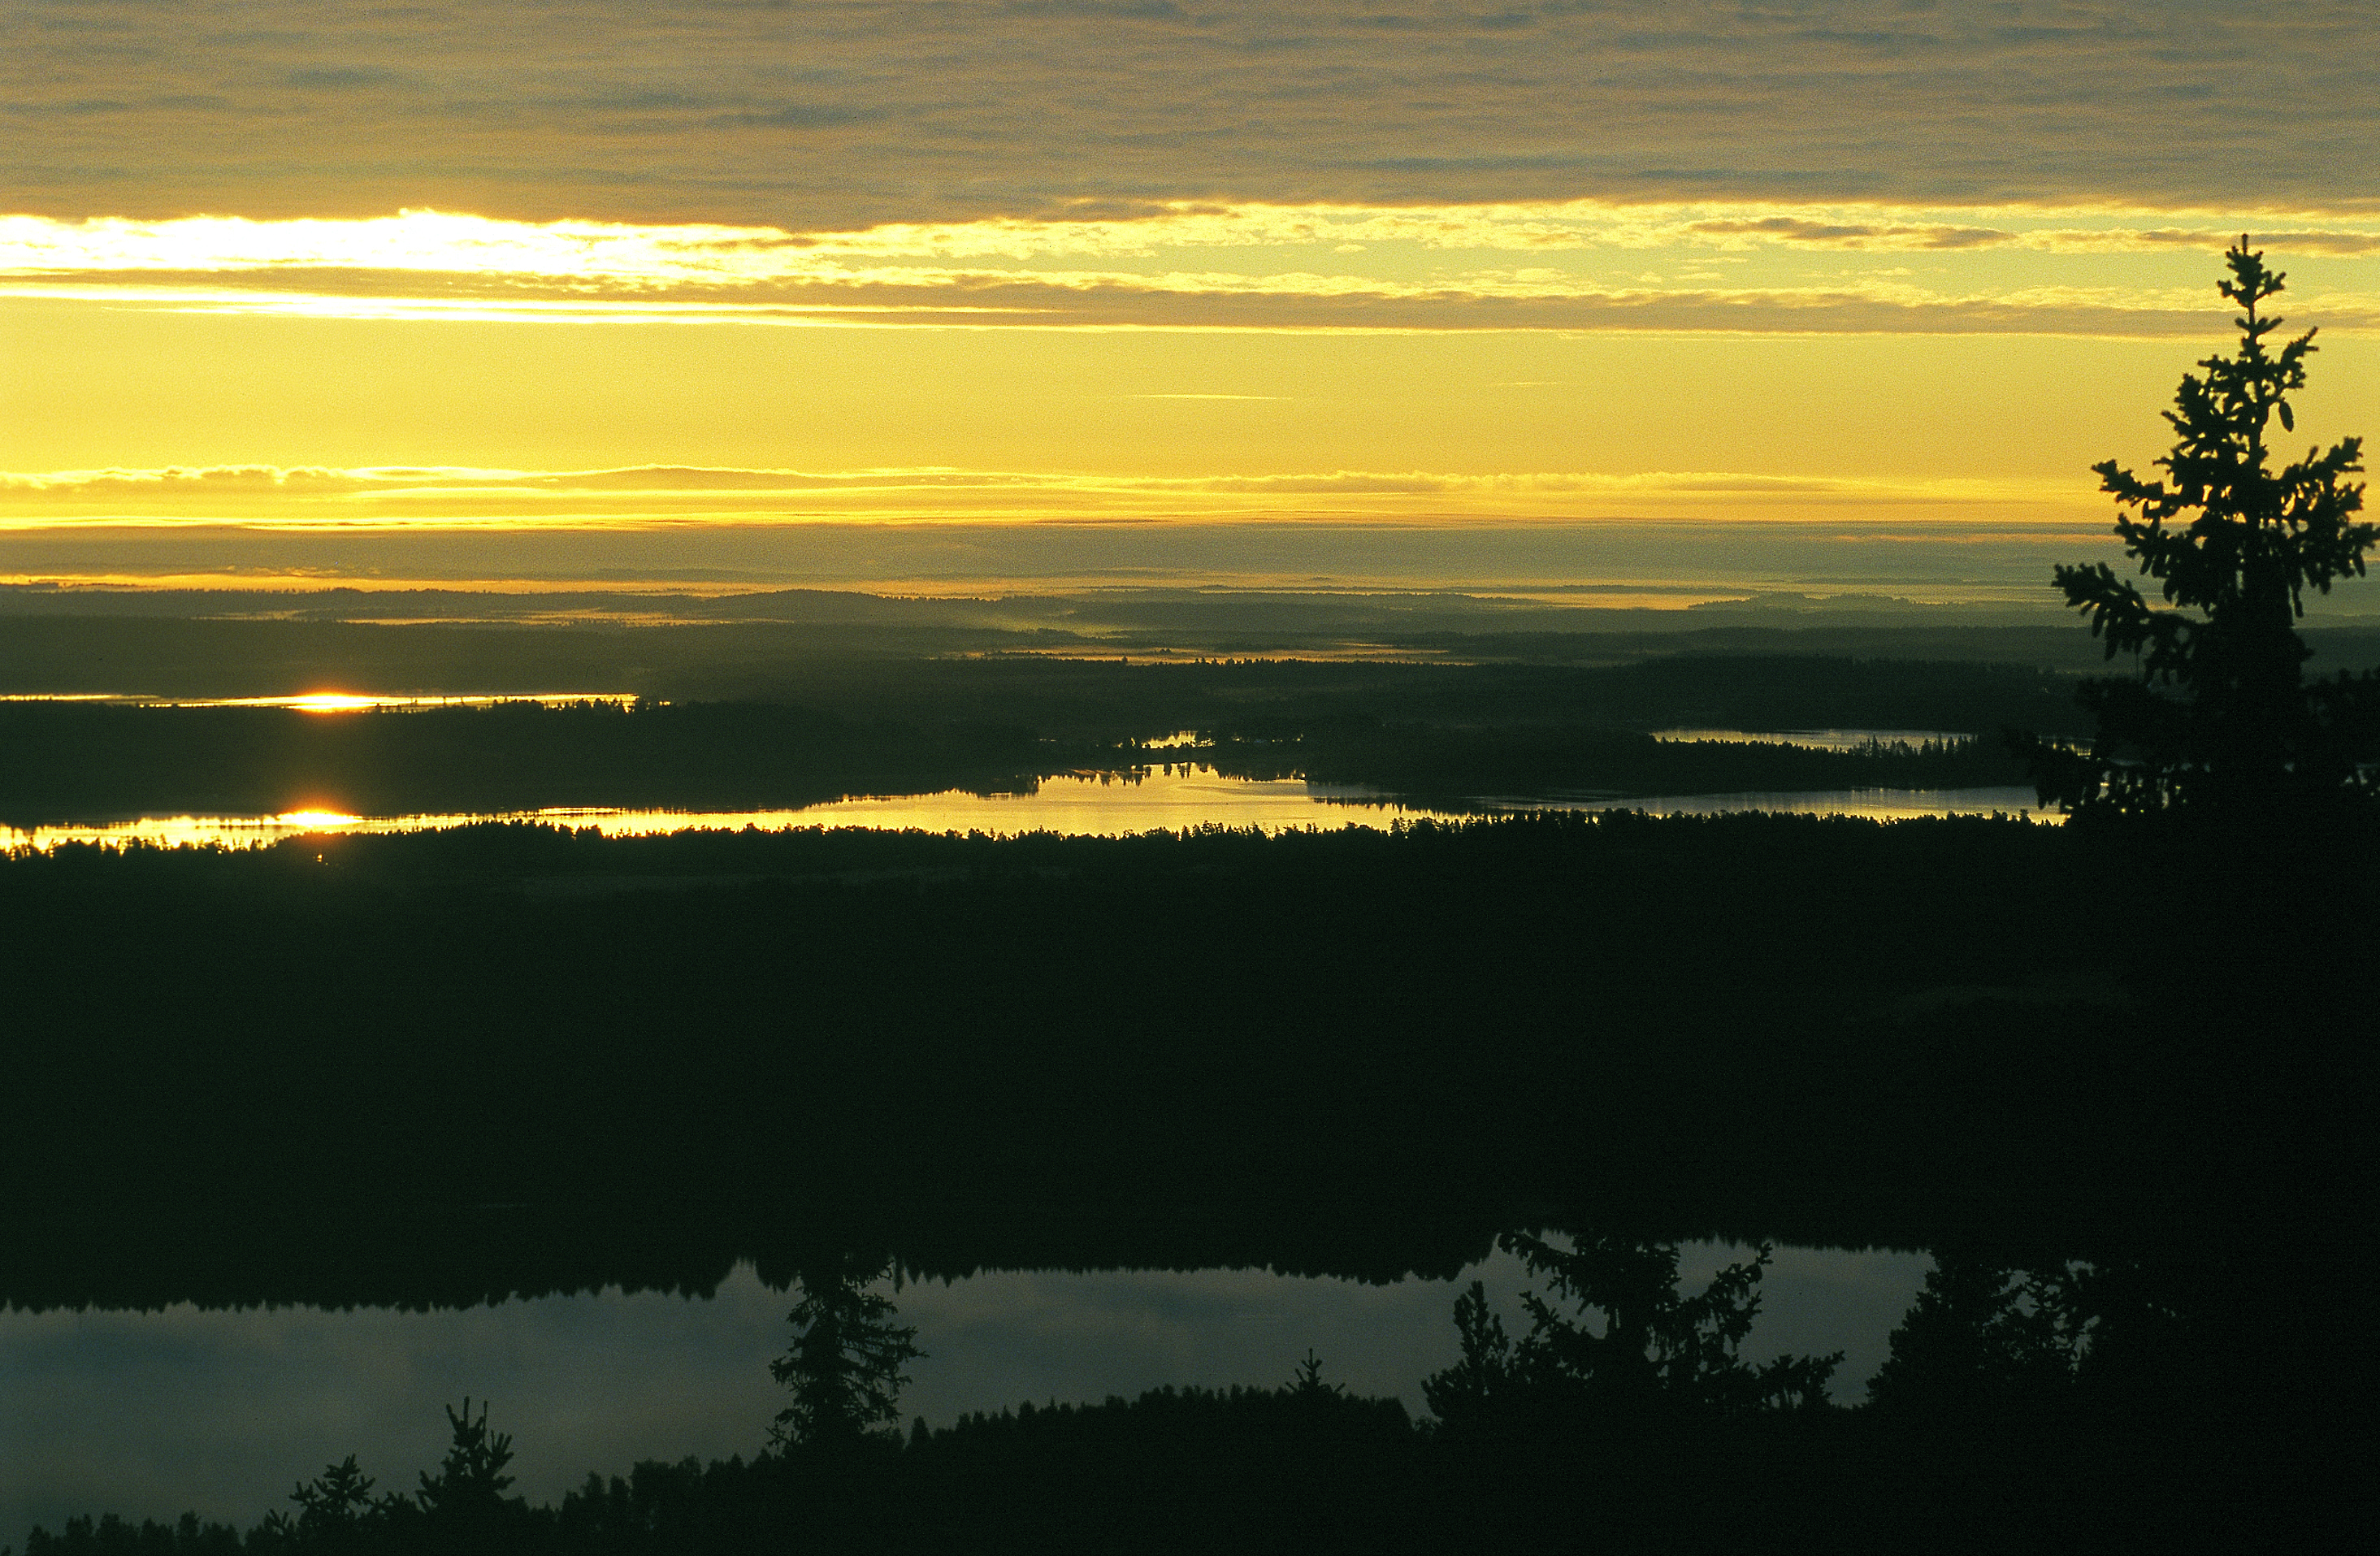
\includegraphics[scale=0.2]{sun.jpg}
	\centering
	\label{fig: sun}

	\caption[Sunset]{An awesome sunset.}
\end{figure}

\faChevronCircleRight\hspace{0.5cm} Einfügen einer Tabelle\\

\faChevronCircleRight
\hspace{0.5cm}
Erstellen smth.







\end{document}
